\documentclass[linenumber]{jdsart}
\usepackage{setspace}
 
\volume{0}
\issue{0}
\pubyear{2022}
\articletype{research-article}
\doi{0000}

\usepackage{siunitx} % For alignment of numbers
\sisetup{
    group-separator = {,},
    round-mode = places,
    round-precision = 2,
    output-decimal-marker = {.},
    table-number-alignment = center,
    table-figures-integer = 6,
    table-figures-decimal = 2,
    table-figures-uncertainty = 2
}


% image path
\graphicspath{{.}{./images}}

\usepackage{xcolor}
%\newcommand{\dt}[1]{\textcolor{purple}{\textbf{DT: (#1)}}}

\let\proglang=\textsf
%% \newcommand{\pkg}[1]{{\fontseries{m}\selectfont #1}}
%% \newcommand\code[2][black]{\textcolor{#1}{\texttt{#2}}}
% Preamble:
\newcommand{\numint}[1]{\num[round-mode=none]{#1}}

\usepackage{comment}
\usepackage{subcaption}
\usepackage{booktabs, textgreek}
\usepackage{enumitem}
\usepackage{tikz} % For creating diagrams
\usepackage{hyperref}   % For clickable links and breaking long URLs
\usepackage{url}        % Optional if hyperref is not loaded
\usepackage{fontawesome}
\usepackage{adjustbox} 
\usepackage{multicol} 
\usepackage{tabularx} 
\usetikzlibrary{positioning} % Required for relative positioning (e.g., "of" keyword)
\captionsetup[subfigure]{justification=centering, font=small}

% Improve figure/table placement discipline
\renewcommand\topfraction{.9}
\renewcommand\bottomfraction{.8}
\renewcommand\textfraction{.07}
\renewcommand\floatpagefraction{.85}
\setcounter{totalnumber}{5}
\setcounter{topnumber}{3}
\setcounter{bottomnumber}{3}



\begin{document}

%\doublespacing 

%\tableofcontents % Optional: Table of Contents
%\listoffigures % List of Figures
%\listoftables % List of Tables


\begin{frontmatter}
  
\title{Detecting Data Anomalies in Open Data: A Case Study with the New
York City 311 Service Request Dataset}
\runtitle{Searching for Data Anomalies}

\author[1]{\inits{D.}\fnms{David}~\snm{Tussey}}
\address[1]{\institution{NYC \textsc{DoITT}}, \cny{USA}}

\begin{abstract}
The open data movement has transformed governance by promoting transparency,
innovation, and public engagement. Since the 2012 Open Data Law, the City of
New York (NYC) has been a leader, publishing over  
\num[round-precision=0]{3000}
datasets through its Open Data portal. Yet the value 
of open data depends on its quality—a topic often overlooked in the literature.

This paper presents a case study of anomaly detection within the popular NYC
311 Service Request (SR) dataset. The analysis reveals that
uncritical reliance on open datasets can yield misleading results.
Detecting these anomalies required custom software and iterative
exploration to uncover patterns not immediately evident.

Rather than cleansing the data, this study characterizes them, while emphasizing
that some anomalies cannot be judged invalid without context. The findings 
highlight the analytical rigor and interpretive judgment necessary to ensure
credible insights from open data.
\end{abstract}

\begin{keywords}
  \kwd{Data anomalies}
  \kwd{Anomaly detection}
  \kwd{Data quality}
  \kwd{Data validation}
  \kwd{Data curation}
  \kwd{Data cleansing}
  \kwd{Data science}
  \kwd{NYC Open Data}
  \kwd{Smart city}
  \kwd{Transparency}
  \kwd{Government data}
\end{keywords}

\end{frontmatter}

\hyphenpenalty=10000
\exhyphenpenalty=10000
\emergencystretch=1em

%-------------------------------------------------------------------------------
%	Section: Introduction
%-------------------------------------------------------------------------------

\section{Introduction}
\label{sec:intro}
The open data movement, emerging in the early twenty-first century, rests on
the premise that freely accessible information can transform governance and
society by fostering transparency, innovation, and civic engagement.
A major milestone was the launch of the U.S.\ \textsc{Data.gov} portal in
2009\,\citep{dataGov}, followed by the European Union’s
\textsc{Open Data Portal} in 2012\,\citep{dataEU}, and the World Bank’s
\textsc{Open Data} initiative in 2010\,\citep{dataWorldBank}.
Together, these efforts democratized access to government information and
encouraged data-driven inquiry across disciplines
\citep{barns2016mine,wang2016adoption}. Yet the effectiveness of open data
depends not merely on access but on quality, consistency, and usability—issues
that remain only partly resolved or addressed.

NYC has been a municipal leader in this arena since the
\textsc{Open Data Law} of 2012\,\citep{zuiderwijk2014open}, which established
the \textsc{NYC Open Data Portal}\,\citep{dataNYC}.
Hosting more than \num[round-mode=none, group-minimum-digits=5]{3000}
datasets across roughly ninety agencies, the portal
has enhanced governmental transparency and supported extensive research in
fields such as public health\,\citep{cantor2018facets,shankar2021data}, urban
development\,\citep{neves2020impacts}, and transportation\,\citep{gerte2019understanding}.
Datasets on restaurant inspections, traffic collisions, and educational
enrollment, among others, have informed both public policy design and civic
applications. In particular, NYC’s 311 SR data have
been used to optimize resource allocation and improve emergency response,
demonstrating their operational value.

The size and diversity of these datasets pose persistent challenges
for data curation—processes that ensure accuracy, completeness, and
coherence across time and sources. High-quality curation also underpins
effective machine-learning models and statistical analyses
\citep{polyzotis2019data,jain2020overview}, while inadequate practices can
introduce bias and undermine decision-making
\citep{geiger2020garbage,rahm2000data}. Although open data initiatives
emphasize dissemination, the burden of verifying and cleaning data often falls
to end users\,\citep{cody2017cody,van2018statistical}. This dynamic is evident
in the 311~SR dataset, where substantial data cleansing is required before
subsequent analysis can proceed.

Research on data curation has advanced understanding of these challenges.
\citet{witt2009constructing} introduced data-curation profiles for specific
research contexts, \citet{borgman2012conundrum} examined governance and
sustainability issues, and \citet{hart2016ten} articulated general principles
for effective management. Empirical studies further illustrate the value of
well-curated data in addressing public-health and crisis-response problems
\citep{cantor2018facets,shankar2021data}. Yet large-scale municipal datasets
remain under-analyzed with respect to systematic quality assessment.

This study addresses that gap through a case analysis of the NYC 311
non-emergency Service Request dataset. Rather than attempting to cleanse or
correct records, this investigation focuses on detecting and characterizing
anomalies that may compromise analytical validity. This approach required
custom software, iterative exploration, and methodological rigor to uncover
patterns not readily visible through routine inspection. Building on these
findings, this paper proposes practical principles for anomaly detection and
data assessment tailored to government-released open data, with the goal of
enhancing reliability, reproducibility, and interpretability in research and
policy contexts.

Section~\ref{sec:service} reviews the history of the NYC 311 system and its
role as a data source, Section~\ref{sec:data} describes the dataset analyzed,
Section~\ref{sec:anomalies} details the principal data-quality issues, and
Section~\ref{sec:principles} outlines recommended curation principles.
Section~\ref{sec:conclusion} concludes with key findings and implications for
future open-data initiatives.

%-------------------------------------------------------------------------------
% Section: NYC 311 Service Request (SR) Data
%-------------------------------------------------------------------------------

\section{The New York City 311 Non-Emergency Service}
\label{sec:service}
The NYC~311 non-emergency service, a cornerstone of the City’s overall service
response framework, provides a single, unified point of contact for requests,
complaints, and inquiries that previously required navigating a maze of
agency-specific phone numbers and reporting processes. Launched in 2003, the
system streamlined access to services ranging from noise issues handled by the
New York Police Department (NYPD) to street maintenance overseen by the
Department of Transportation (DOT) to rodent reports investigated by the
Department of Health and Mental Hygiene (DOHMH), reducing confusion for
residents and misrouting for agencies. Initially limited to phone calls, the
311 system has expanded to include a mobile application, web portal, text
messaging, social media, and chat support. Over two decades, NYC~311 has
evolved into a comprehensive data management platform processing more than
\num[round-precision=0]{3} {million} SRs annually, with 2025 on track to set a
record of \SI{3.48	}{million} SRs.


Beyond its operational function, NYC 311 data are instrumental in shaping
City governance and community engagement. Open data enhance transparency while
empowering civic developers, policymakers, and the public
\citep{minkoff2016nyc,o2017uncharted,kontokosta2021bias}. These data have
informed crisis management (e.g., directing residents to shelters during
emergencies or extreme weather events, and coordinating COVID-19 responses),
improved everyday urban governance (e.g., landlord–tenant enforcement, taxi
route realignment by the Taxi and Limousine Commission (TLC), rodent control,
and agency responsiveness), and supported a range of academic studies on urban
issues, including resource allocation\,\citep{zha2014profiling,raj2021swift},
social equity in service provision\,\citep{white2018promises,kontokosta2021bias},
environmental challenges\,\citep{dove2022sounds}, and street flooding
\,\citep{agonafir2022understanding}.

%-------------------------------------------------------------------------------
% Section: 311 SR Dataset Description
%-------------------------------------------------------------------------------

\section{Dataset Description}
\label{sec:data}
This study uses a five-year dataset (2020--2024) of NYC 311 SRs, downloaded
from the NYC Open Data Portal on 2025-10-10. The dataset’s main characteristics
are:

\begin{itemize}[left=1.5em]
\item The raw dataset consists of 16~million records (9~GB) in CSV
format. For efficiency in the R programming environment, the file was converted
to the RDS format. Each record has 41~fields, with each row
representing a single SR (e.g., complaint, issue, or request).

\item Four date fields use \texttt{YYYY-MM-DD HH:MM:SS} format:\\
\texttt{created\_date}, \texttt{resolution\_action\_updated\_date}, \texttt{due\_date},
 and \texttt{closed\_date}.

\item Two borough fields, \texttt{borough} and \texttt{park\_borough}, appear
to duplicate one another.

\item Seven street-related fields are included, with two pairs of apparent
duplicates:\\
\texttt{incident\_address}, \texttt{street\_name}, \texttt{landmark};
\texttt{cross\_street\_1} and \texttt{cross\_street\_2};
\texttt{intersection\_street\_1} and \texttt{intersection\_street\_2}.

\item Eight incident location fields are included (two of which are geocoded):\\
\texttt{incident\_address}, \texttt{latitude} and \texttt{longitude},
\texttt{location} (a concatenation of latitude and longitude),
\texttt{street\_name}, \texttt{landmark}, \texttt{block}
(NYC tax-lot mapping), \\
\texttt{x\_coordinate\_state\_plane},
 and  \texttt{y\_coordinate\_state\_plane} (a coordinate system 
 developed by NOAA's National Geodetic Survey.)
\end{itemize}

Table~\ref{tab:big-six-agencies} summarizes the volume distribution across the
largest contributing agencies.

\begin{table}[tbp]
  \centering
  \caption{Top six agencies by share of SRs (2020--2024).}
  \label{tab:big-six-agencies}
  \begin{tabular}{lrr}
    \toprule
    \textbf{Agency} & \textbf{Abbreviation} & \textbf{Share of \textsc{SRs}} \\
    \midrule
    New York Police Department & NYPD & 43\% \\
    Housing Preservation and Development & HPD & 19\% \\
    Department of Sanitation & DSNY & 12\% \\
    Department of Transportation & DOT & 7\% \\
    Department of Environmental Protection & DEP & 5\% \\
    Department of Parks and Recreation & DPR & 4\% \\
    \midrule
    \textbf{Total (Top Six)} &  & \textbf{90\%} \\
    \bottomrule
  \end{tabular}
\end{table}

The dataset contains 252 distinct \texttt{complaint\_type} categories with
the top twenty complaints account for \SI[round-precision = 2]{68.46}{\percent}of all SRs. The
complaint distribution is highly skewed, with a small number of issues
dominating overall volume and a long tail of low-frequency complaints.

Noise-related complaints are especially prominent, represented by eight
separate categories, including vehicle, residential, commercial, helicopter,
and street/sidewalk noise. Taken together, these account for nearly one-quarter
(\SI[round-precision = 1]{23.4}{\percent}) of all complaints, making
\emph{noise} by far the most common NYC complaint. Other leading categories
include illegal parking, heat/hot water complaints, blocked driveway, and plumbing.

Anomalies in the dataset are also typically associated with specific City
agencies, which often facilitates targeted corrective actions. For example,
some anomalies occur in only one agency, enabling precise remediation.
As shown in Table~\ref{tab:big-six-agencies}, the six largest agencies account
for \SI[round-precision = 0]{90}{\percent} of all SRs submitted between 2020 and 2024.

%-------------------------------------------------------------------------------
% Section: Data Cleansing Issues and Anomalies
%-------------------------------------------------------------------------------

\section{Data Cleansing and Anomaly Identification}
\label{sec:anomalies}
Data cleansing is the process of identifying and correcting errors,
inconsistencies, anomalies, and inaccuracies to ensure that a dataset is
sufficiently reliable for analysis\,\citep{maletic2005data,hosseinzadeh2023data}.
Typical operations include removing duplicates, handling missing values,
correcting mislabeled entries, and standardizing formats
\,\citep[e.g.,][]{cody2017cody,van2018statistical}. For open data, these
challenges are amplified by the diversity of sources and the lack of
coordination across contributing agencies, leading to uneven quality and
consistency. When data cleansing is achieved, it enhances trust, supports
reliable analysis, and facilitates integration into applications such as
machine learning.

This study does not attempt to cleanse the NYC 311 dataset but instead focuses
on the preceding step—systematically detecting and characterizing anomalies
that may compromise its reliability.

%-------------------------------------------------------------------------------
% Sub-section: Pre-analysis Data Modifications
%-------------------------------------------------------------------------------

\subsection{Pre-analysis Data Modifications}
\label{subsec:premodifications}
Prior to analysis, the raw dataset undergoes a series of preparatory
modifications to facilitate efficient processing. These steps include both
structural adjustments and content standardization:

\begin{itemize}[left=1.5em]
  \item \textbf{Standardization of structure:}
  Column names are normalized for ease of reference, and the raw
  \texttt{.csv} file is converted into the more efficient \texttt{.rds} format
  to improve performance.

  \item \textbf{Date handling:}
  All date fields are converted to the \texttt{POSIXct} class and aligned
  to the \textit{America/New\_York} time zone, enabling accurate
  treatment of Daylight Saving Time (DST) effects (discussed in
  Section~\ref{par:dst}).

  \item \textbf{Agency harmonization:}
  Several agencies were renamed during the study period; records were
  consolidated under their current agency designations for consistency and
  accuracy.

  \item \textbf{Validation of completeness:}
  Rows are screened for mandatory fields. Missing or absent values—
  recorded in multiple raw formats—are standardized to \texttt{NA} to
  facilitate processing. 

  \item \textbf{Field formatting:}
  Text fields are converted to uppercase for consistent matching, and
  numeric fields are explicitly cast to the appropriate type.
\end{itemize}

%-------------------------------------------------------------------------------
% Sub-section: Structural Issues
%-------------------------------------------------------------------------------

\subsection{Structural Issues}
\label{subsec:structural}
Structural issues concern the way data are organized, formatted, or
encoded—that is, how the dataset is \emph{structured} rather than what it
\emph{contains}. Structural issues can hinder efficient analysis and often
require substantial preprocessing before the data can be reliably used. In the
NYC 311 dataset, three notable structural issues were identified:

\begin{itemize}[left=1.5em]
  \item inconsistent representation of missing-data values,
  \item Daylight Saving Time (DST) anomalies, and
  \item precision versus accuracy issues in the \texttt{latitude},
  \texttt{longitude}, and \texttt{location} fields.
\end{itemize}

\paragraph{Inconsistent Representation of Missing Data}
\label{par:missingdata}
The NYC 311 dataset exhibits inconsistent conventions for representing
missing values. Observed forms include nulls, blank spaces, ``\texttt{NA}'',
``\texttt{N/A}'', and ``\texttt{<NA>}'’. Such variation complicates
programming and analysis, increasing the likelihood of errors when filtering
or aggregating records. To address this issue, all missing values were
standardized to \texttt{NA}. Notably, nearly one-fifth 
(\SI[round-precision = 2]{17.97}{\percent}) of the 
dataset contains missing entries.

\paragraph{Daylight Saving Time Issues}
\label{par:dst}
The NYC 311 dataset records timestamps in New York City local time, which
observes Daylight Saving Time (DST). Twice each year, this practice
introduces temporal discontinuities that affect the calculation of SR
durations, defined as the difference between \texttt{closed\_date} and
\texttt{created\_date}.

During the spring transition, local clocks advance from 01:59:59 directly to
03:00:00, eliminating the entire hour between 02:00:00 and 02:59:59. As a
result, durations of SRs created shortly before the transition and closed
 afterward has their durations exaggerated by up to one hour.

During preprocessing, several date fields were found to violate the DST
spring-forward rule, with timestamps recorded during the nonexistent hour
between 02:00:00 and 02:59:59
(e.g., \texttt{2024-03-10 02:00:46},
\texttt{2020-03-08 02:10:00}). Such values are invalid, as local time
advances directly from 01:59:59 to 03:00:00 on those dates. These anomalies
were corrected by shifting the affected timestamps forward to valid times
(e.g., \texttt{2024-03-10 03:00:46},
\texttt{2020-03-08 03:10:00}). In total, nineteen such corrections were made.

The fall DST adjustment introduces a more serious systemic issue by producing
SRs with \emph{negative} durations, where the \texttt{closed\_date} precedes
the \texttt{created\_date}. Such cases are logically impossible and can
distort agency-level performance measures, particularly for time-sensitive SRs.
The following example illustrates the problem:

\begin{itemize}[left=1.5em]
  \item A residential noise complaint is created at 01{:}50 on Sunday,
  2024-11-03, the date of the DST fallback transition.

  \item The NYPD responds promptly, resolving the issue in forty minutes.  
  Without DST adjustments, the resolution would normally be recorded at
  02{:}30.

  \item However, during this interval the local clock is set back one hour, so
  the resolution is time-stamped as 01{:}30.

  \item As a result, the 311 system records the SR as closed twenty minutes
  \emph{before} it was created, yielding a nonsensical negative duration of
\num{-20}~minutes.
\end{itemize}

On average, \numint{86} SRs per year exhibit this systemic issue, 
with a mean negative duration of \SI[round-precision = 2]{42.24}{\percent} . 
Although rare, these anomalies can disproportionately affect 
time-sensitive complaint categories such as
\texttt{drug\_activity}, \texttt{homeless\_assistance}, and
\texttt{disorderly\_youth}, and they can distort aggregate performance metrics.
Even a small number of implausible durations can shift summary statistics and
obscure true operational patterns.


\paragraph{Precision versus Accuracy in Latitude/Longitude Values}
\label{par:precision}
The \texttt{latitude}, \texttt{longitude}, and the duplicative \texttt{location}
fields in the raw dataset exhibit substantial variation in numeric precision.
The majority (\SI[round-precision = 2]{90.23}{\percent} ) of values 
are recorded with thirteen decimal places, (e.g., 
\texttt{latitude} = 40.7022221884127, \texttt{longitude} = -73.9126848719299), 
representing
\SI[round-precision=2]{89.18}{\percent} of \texttt{latitude} and 
\SI[round-precision=2]{90.23}{\percent} of \texttt{longitude} values.
However, the overall precision span extends from eight to fifteen decimals for 
\texttt{latitude} and from zero to fifteen for \texttt{longitude}. A small 
subset of \numint{212} records contains only integer longitude values
with no decimals, highlighting inconsistent data-handling practices.

Such heterogeneity suggests inconsistent data capture rather than deliberate
standardization. Moreover, positional precision at fourteen decimal places
implies spatial resolution at the molecular scale—far beyond any plausible
accuracy for municipal sensors or geocoding. This represents excessive numeric
precision rather than meaningful accuracy.

For reference, the official New York City Borough Boundary (Water Included)
dataset (\textsc{NYBBWI}), published by the Department of City Planning (DCP),
provides coordinates to six decimal places, corresponding to practical
accuracy on the order of a few meters. In the present analysis, the original
coordinates were retained without rounding but were evaluated against the
official city boundary extents in (\textsc{NYBBWI}) using a tolerance of
approximately \SI[round-precision=0]{100}{\meter}.

%-------------------------------------------------------------------------------
% Sub-section: Missing Data by Field
%-------------------------------------------------------------------------------

\subsection{Missing Data by Field}
\label{subsec:blanks}
Understanding the extent and distribution of missing data across fields is
essential for evaluating the overall usability of the dataset. For example,
assessing whether SRs were closed before their \texttt{due\_date} is largely
infeasible, as more than \SI[round-precision=0]{99}{\percent} of entries in the
\texttt{due\_date} field are blank.

Additionally, field usage varies considerably across agencies. For instance,
\texttt{landmark} and \texttt{facility\_type} are widely used across agencies,
underscoring their importance in classifying SRs. By contrast,
\texttt{taxi\_pick\_up\_location} is used exclusively by TLC. Fortunately most
of the fields used in this analysis are well populated.

Table~\ref{tab:completeness-lower} summarizes fields exhibiting moderate or
lower completeness rates.

\begin{table}[tbp]
\centering
\caption{Fields with moderate or incomplete data completeness (2020--2024).}
\label{tab:completeness-lower}
\small
\begin{tabular}{l r r}
\toprule
\textbf{Field} & \textbf{Filled count} & \textbf{Completeness (\%)} \\
\midrule
\texttt{taxi\_company\_borough} & \num[round-mode=none]{8564} & 0.05 \\
\texttt{due\_date} & \num[round-mode=none]{52346} & 0.33 \\
\texttt{vehicle\_type} & \num[round-mode=none]{181533} & 1.13 \\
\texttt{facility\_type} & \num[round-mode=none]{211240} & 1.32 \\
\cmidrule(lr){1-3}
\texttt{landmark} & \num[round-mode=none]{9058628} & 56.56 \\
\texttt{intersection\_street\_1} & \num[round-mode=none]{10251224} & 64.00 \\
\texttt{intersection\_street\_2} & \num[round-mode=none]{10257371} & 64.04 \\
\texttt{cross\_street\_2} & \num[round-mode=none]{11693685} & 73.01 \\
\texttt{cross\_street\_1} & \num[round-mode=none]{11696472} & 73.03 \\
\texttt{address\_type} & \num[round-mode=none]{13246948} & 82.71 \\
\texttt{location\_type} & \num[round-mode=none]{13823312} & 86.31 \\
\texttt{bbl} & \num[round-mode=none]{14128219} & 88.21 \\
\bottomrule
\end{tabular}

  \vspace{6pt}
  \raggedright
  \footnotesize
  Note. Fields below 53\% completeness are classified as \emph{Incomplete or
  sparse}; fields between 53\% and 93\% completeness are classified as
  \emph{Moderately complete}.
\end{table}


%-------------------------------------------------------------------------------
% Sub-section: Validating Data for Compliance with Allowable Values
%-------------------------------------------------------------------------------

\subsection{Validating Data for Compliance with Allowable Values}
\label{subsec:domain}

\paragraph{Validating Data Type}
\label{par:validatingdatatype}
The 311~SR Data Dictionary, last updated in~2023, provides limited information
regarding the data type or class of each field, although most can be
reasonably inferred. The NYC Open Data Portal supplements this documentation
by indicating field types with icons:
\textbf{T}{\scriptsize\textbf{T}} for text, \emph{\textbf{\#}} for numeric,
\faCalendar\ for date or time fields, and \faMapMarker\ for geospatial data.

In most cases, these indicators are sufficient for validation. However, the
\texttt{incident\_zip} field is labeled with the text emblem
(\textbf{T}{\scriptsize\textbf{T}}), even though ZIP codes are best regarded as
fixed-length, numeric but non-computational identifiers.

All fields validated properly against their expected data types, as determined
from the 311~SR Data Dictionary and the NYC Open Data Portal descriptions.
However, analytic work requires more than correct typing. Fields must also
contain values that are valid, bounded, and compliant with a known value
domain. For some attributes, the Data Dictionary specifies those domains
explicitly. For others, the documented domain was incomplete or inaccurate,
and valid values had to be inferred from operational usage, supplemental
documentation, or external datasets. As a result, several anomalies were found
where observed legal values did not align with published specifications.

\paragraph{ZIP Codes}
\label{par:zipcodesissues}
Validation of the \texttt{incident\_zip} field is relatively straightforward,
as the U.S.\ Postal Service (\textsc{USPS}) maintains a definitive database of
\numint{42735} valid ZIP codes. Within the NYC~311 dataset, however,
\numint{3274} entries were found to be invalid, including clearly erroneous values
such as \texttt{00000}, \texttt{00083}, and \texttt{11111}.
Although these represent only \SI[round-precision = 2]{0.02}{\percent} of all
records, the presence of invalid ZIP codes is notable because this field is
among the easiest to validate against an authoritative reference. These
anomalies highlight the importance of automated domain checks, particularly
for fields governed by well-defined external standards.

\paragraph{Community Boards}
\label{sec:communityboardissues}
The \texttt{community\_board} field captures one of New York City’s key units
of local governance. Validation should be straightforward, given a publicly
available list of community boards. Nonetheless, this analysis identified
\numint{56914} (\SI[round-precision = 2]{0.36}{\percent}) invalid entries, 
representing values outside the accepted set. Such
anomalies underscore the risks that emerge when categorical fields linked to
administrative structures are not systematically validated.

%-------------------------------------------------------------------------------
% Sub-section: Date Field Issues
%-------------------------------------------------------------------------------

\subsection{Date Field Issues}
\label{subsec:datefieldissues}
In addition to the DST-related structural anomalies discussed in
Section~\ref{par:dst}, the dataset exhibits further temporal issues.
Fundamentally, dates should follow a logical sequence. The
\texttt{created\_date} should precede the \texttt{closed\_date}, and
intermediate timestamps (e.g., \texttt{due\_date}) should plausibly fall
between these events. The NYC~311 dataset includes four such fields:
\texttt{created\_date}, \texttt{due\_date}, \texttt{resolution\_action\_updated\_date}, and
\texttt{closed\_date}. In practice, numerous records violate these expected
relationships, complicating both analysis and interpretation.

\subsubsection{Created Date}
\label{subsubsec:createddate}
All \texttt{created\_date} values were checked to ensure that none were set in
the future or before the inception of the 311 system (circa~2003); all records
were compliant. However, a notable clustering of timestamps occurs at exactly
midnight (\numint{14409} cases) and exactly noon (\numint{31872} cases), an anomaly
examined further in Section~\ref{subsubsec:midnightnoonissues}.

\subsubsection{Due Date Anomalies}
\label{subsubsec:duedate}
The \texttt{due\_date} field appears almost exclusively in Department of
Sanitation (\textsc{DSNY}) records and is populated in only about
\SI[round-precision = 1]{0.3}{\percent} of cases. All values passed validation
(no implausibly past or future dates), and no unusual patterns were seen.

Sixteen cases were found where the \texttt{due\_date} precedes the
\texttt{created\_date}—a nonsensical condition. These ranged from just over
one year early to more than two years early. While these anomalies are few and
unlikely to materially affect aggregate results, they must be excluded to
avoid distorted deadline-performance analyses.

\subsubsection{Closed Date}
\label{subsubsec:closeddate}
Most records were compliant with respect to temporal bounds; none were set
before 2003 or in the future. However, there is a clustering of 
timestamps at exactly 
midnight (\numint{1083862}; \SI[round-precision = 2]{6.77}{\percent}) 
of non-missing \texttt{closed\_date}(s)) and exactly noon
(\numint{294817}; \SI[round-precision = 2]{1.84}{\percent}) representing
 a significant artifact, discussed further in
Section~\ref{subsubsec:midnightnoonissues}. Additionally, \numint{45,296} entries
show \texttt{closed\_date}(s) preceding \texttt{created\_date}(s); these
negative durations are examined in detail in
Subsection~\ref{subsec:duration}.

\subsubsection{Resolution Action Updated Date}
\label{subsubsec:resolutionupdatedate}
The \texttt{resolution\_action\_updated\_date} field records modifications or
follow-up actions related to an SR. No values were found in implausible years.
However, \numint{374974} entries
(\SI[round-precision = 2]{2.34}{\percent}) occur before the corresponding
\texttt{created\_date}. Nearly Nearly \SI[round-precision=0]{80}{\percent} occur within a day occur within a day (often
within seconds), suggesting automated prepopulation during early processing
pipeline stages rather than genuine updates.

A more consequential irregularity concerns post-closure updates.
Approximately (\SI[round-precision=0]{54}{\percent}) of updates occur after the
\texttt{closed\_date}, which is reasonable. However, \numint{27810} entries occur
more than 30~days—up to \numint{1593}~days (over four years)—post closure. A Pareto
analysis indicates that over \SI[round-precision=0]{85}{\percent} of these very 
late updates are concentrated in TLC, DPR, and DOHMH. Determining 
whether such delays reflect administrative workflows or 
erroneous logging warrants further attention.

Finally, 91 records exhibit extremely late post-closure updates where
invalid \texttt{closed\_date} values (i.e., 1899–1900) trigger an artificially large
duration. This behavior is consistent with the well-known SQL default-date
placeholder for null datetimes, and a similar behavior can arise in Microsoft Excel.
These records should be excluded to prevent severe distortions in statistical
summaries, as illustrated in Table~\ref{tab:extreme-positive-days-agency}.

\subsubsection{Daylight Saving Time (DST) Anomalies}
\label{subsubsec:dst}
As discussed in Section~\ref{par:dst}, DST introduces systemic measurement
errors. The fallback adjustment yields implausible negative durations in
averaging \num{86} SRs per year   mean negative duration of \SI{-42.24}{\minute}, 
while the spring-forward adjustment inflates durations for 
approximately \numint{55000} SRs annually due to the missing 02{:}00–02{:}59 interval.

Although offsets of \SI{+1}{\hour} or \SI{-42}{\minute} may seem minor, such
systematic distortions can notably affect performance metrics for
time-sensitive complaints such as \texttt{Noise--Residential},
\texttt{Animal--Abuse}, \texttt{Homeless~Person~Assistance}, and
\texttt{Drug~Activity}. These artifacts underscore the importance of
properly accounting for DST when computing SR durations.

\subsubsection{Midnight and Noon: Creation and Closure Issues}
\label{subsubsec:midnightnoonissues}
SR activity generally follows a typical diurnal pattern, with most requests
created during daytime hours.

Closer examination of the \texttt{created\_date} and \texttt{closed\_date}
fields reveals substantial peaks exactly at midnight (00{:}00{:}00) and noon
(12{:}00{:}00). These alignments are unlikely to result from human activity
and instead suggest automated batch operations closing or initializing large
numbers of SRs at these times. Although not erroneous per se, such artifacts
can distort hourly workload profiles and performance indicators.

As shown in Figure~\ref{fig:exacthours}, both created and closed timestamps
display pronounced concentrations at these precise times, far exceeding random
expectation and surpassing a \(+3\sigma\) threshold.

\begin{figure}[tbp]
  \centering
  \begin{subfigure}[b]{0.49\textwidth}
    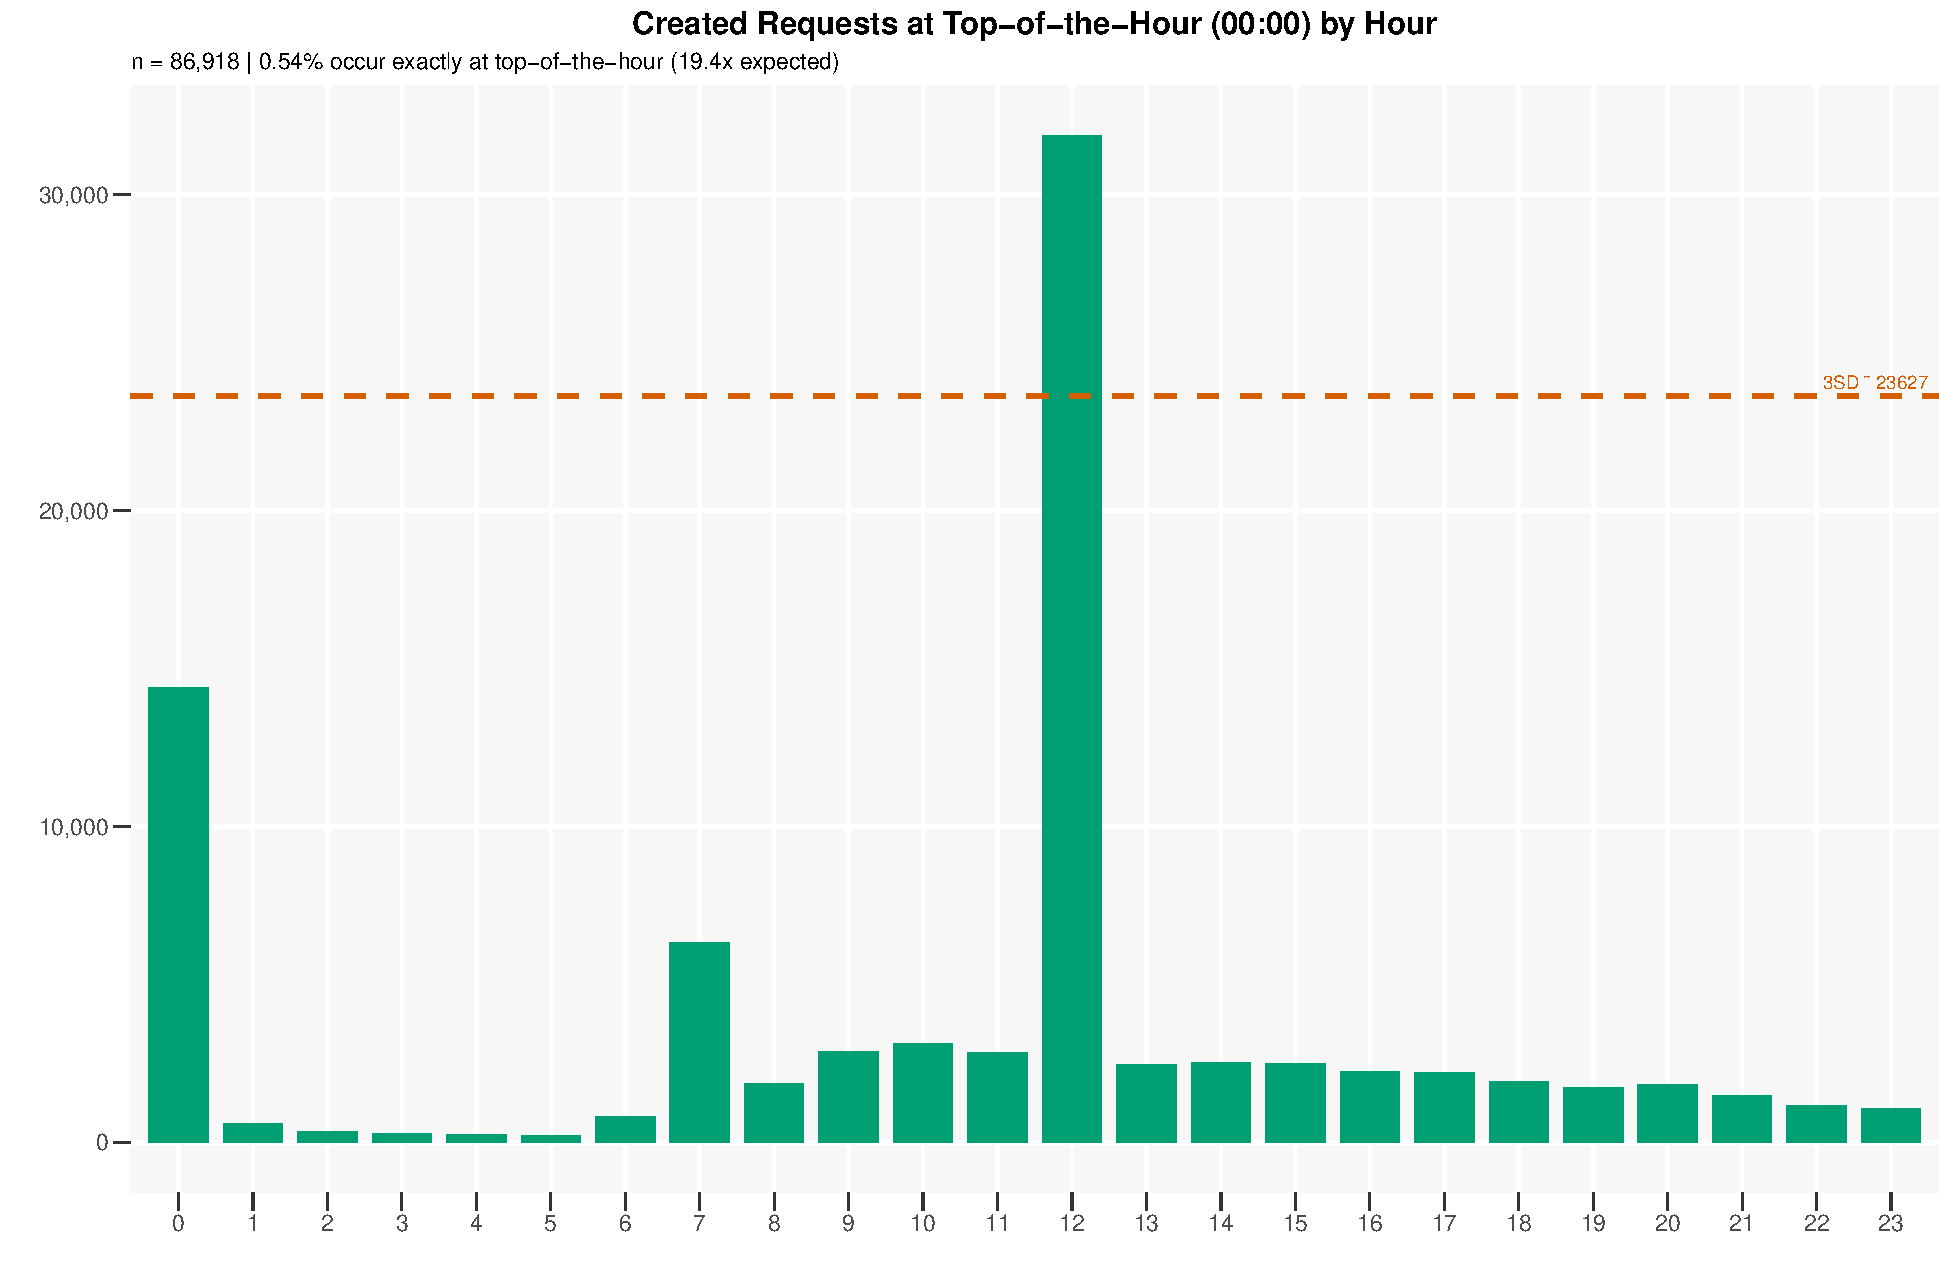
\includegraphics[width=\textwidth]{created_top_of_hour_distribution.pdf}
    \caption{\textsc{SR}s created at the top of the hour.}
    \label{fig:created_top_hour}
  \end{subfigure}
  \hfill
  \begin{subfigure}[b]{0.49\textwidth}
    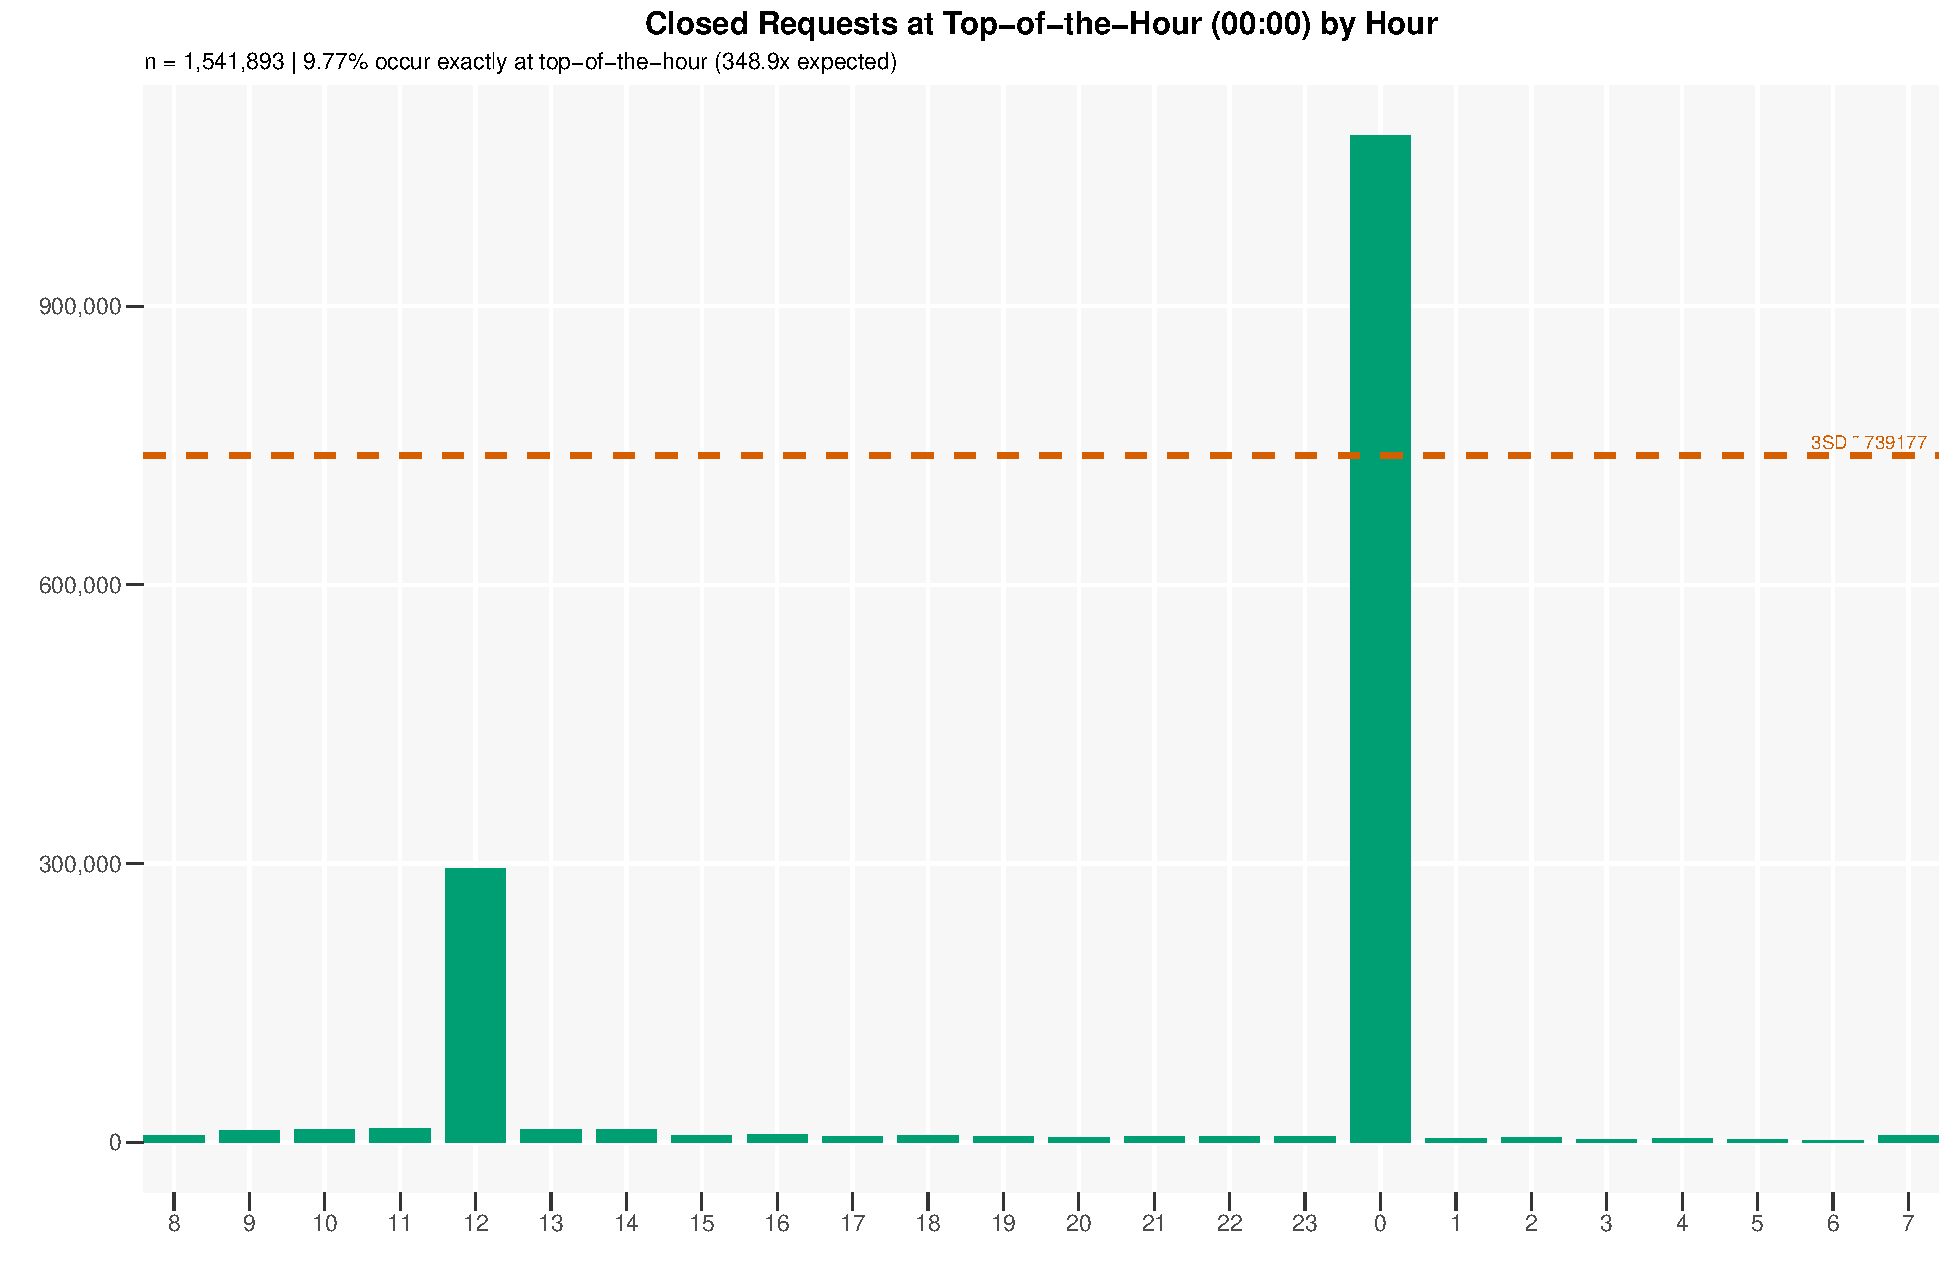
\includegraphics[width=\textwidth]{closed_top_of_hour_distribution.pdf}
    \caption{\textsc{SR}s closed at the top of the hour.}
    \label{fig:closed_top_hour}
  \end{subfigure}
  \caption{311~\textsc{SR}s created and closed exactly at the top of the hour (HH{:}00{:}00).}
  \label{fig:exacthours}
\end{figure}

%-------------------------------------------------------------------------------
% Sub-section: Duration Issues
%-------------------------------------------------------------------------------

\subsection{Duration Issues}
\label{subsec:duration}
The lifespan of an SR—its \emph{duration}—is widely used as a performance
metric for NYC agencies. Duration informs assessments of equity in service
provision across neighborhoods and boroughs, and serves as a proxy for agency
responsiveness in formal reporting. Given this importance, SR duration
warrants close scrutiny.

In principle, duration is the elapsed time between
\texttt{created\_date} and \texttt{closed\_date}. Given the prevalence of
automated workflows, these timestamps might be expected to be populated
programmatically in response to user actions—reducing potential errors and
enforcing temporal coherence. However, this is not always the case. The
dataset includes several anomalies in these fields that would ordinarily be
prevented by robust automation, raising concerns about the reliability of
duration as a performance indicator.

\subsubsection{Negative Durations}
\label{subsubsec:negativedurations}
A total of \numint{45296} SRs exhibit a \texttt{closed\_date} that precedes the
\texttt{created\_date}, producing nonsensical negative durations. Across all
affected SRs, negative durations average \SI[round-precision=1]{-118.7}{\day}, a nontrivial distortion
that varies considerably by agency (Table~\ref{tab:negative-days-agency}).

Within this group, \numint{115} SRs show \emph{extreme} negative durations due to default
\texttt{closed\_date} values in 1899 and 1900—implying durations exceeding
\num{-122}~years. Such outliers can dramatically skew summary statistics,
making mean calculations unreliable without adjustment.

Negative durations are overwhelmingly concentrated within the
DOT which accounts for approximately (\SI[round-precision=0]{98}{\percent}) 
of all cases. This uneven distribution suggests that the
anomaly reflects systemic or procedural issues rather than random noise. If
left unaddressed, these errors would severely distort any downstream analysis
relying on duration metrics.

\begin{table}[tbp]
\centering
\caption{Negative Duration (days) by agency}
\label{tab:negative-days-agency}
\begin{tabular}{l
  S[table-format=5.0, round-mode=places, round-precision=0]
  S[table-format=3.2]
  S[table-format=3.2]
  S[table-format=3.2]
  S[table-format=3.2]
  S[table-format=3.2]
  S[table-format=3.2]}
\toprule
\textbf{Agency} &
\textbf{N} &
\textbf{Min} &
\textbf{Q1} &
\textbf{Median} &
\textbf{Q3} &
\textbf{Max} &
\textbf{Mean} \\
\midrule
NYPD  & 431   & -0.08  & -0.06  & -0.02  & -0.01  & 0.00   & -0.03 \\
HPD   & 320   & -1.27  & -0.48  & -0.37  & -0.29  & 0.00   & -0.37 \\
DOB   & 37    & -0.84  & -0.53  & -0.48  & -0.39  & -0.08  & -0.47 \\
DOT   & 44143 & -378.00 & -5.00 & -2.96 & -1.14 & 0.00 & -5.51 \\
DSNY  & 18    & -27.52 & -4.99 & -4.97 & -1.88 & -1.50 & -6.44 \\
DEP   & 228   & -548.76 & -405.59 & -316.21 & -210.58 & -1.22 & -292.36 \\
\bottomrule
\end{tabular}
\end{table}

\subsubsection{Zero and One-Second Durations}
\label{subsubsec:zerodurations}
A more prevalent anomaly occurs when \texttt{closed\_date} and
\texttt{created\_date} share the exact same timestamp, producing zero-duration
SRs. A total of \numint{387329} SRs (\SI[round-precision = 2]{2.5}{\percent}) fall
into this category. In addition, \numint{3460} SRs close within one second of their
creation. While not logically impossible, these near-instantaneous resolutions
are highly improbable. Moreover, \SI[round-precision = 0]{81}{\percent} 
of such cases originate
from just three agencies (DOHMH, DOT, and Department of Buildings (DOB), 
indicating agency-specific workflows or system-level artifacts.

\subsubsection{Suspicious Durations}
\label{subsubsec:suspiciousdurations}
\textbf{Rationale.}
SR durations are highly right-skewed, with some cases extending months or
years. Such extremes distort summary measures and hinder comparisons across
agency workloads. Accordingly, a statistical analysis was undertaken to 
determine appropriate lower-bound thresholds for identifying implausible 
duration values.

\textbf{Methodology.}
Durations were truncated to plausible limits: 2~seconds (excluding
zero- and one-second artifacts) to \numint{172800}~seconds (48~hours). This reduced
the dataset from 15.3~to~10.0~million records (\SI[round-precision = 2]{64.9}{\percent}
retained), and greatly shortened the long tail. Five complementary outlier
screening methods were evaluated: standard deviation (SD), median absolute
deviation (MAD), log-normal thresholds, percentile cutoffs (1–10\%), and
interquartile range (IQR).

\textbf{Findings.}
Truncation reduced the mean-to-median ratio from~53.7~to~5.2. SD, 
MAD, and IQR tests did not flag further anomalies. Log-normal and 
percentile methods produced operationally reasonable limits. 
The adopted rule—a log-normal $+3\sigma$ cutoff (\SI{27.95}{\second})—balanced 
rigor and interpretability, identifying only \SI[round-precision = 2]{0.07}{\percent} 
of remaining records as outliers (\numint{14741} cases) with questionable or suspicious
durations..

\textbf{Summary.}
Combining zero durations (\numint{387329}), one-second durations (\numint{1240}), and
suspicious durations under 28~seconds (\numint{14471}), a total of \numint{403310}~SRs
(\SI{2.6}{\percent} ) are statistically suspicious or operationally implausible.

\subsubsection{Positive Durations}
\label{subsubsec:positivedurations}
While a positive duration is not inherently erroneous, a subset of SRs exhibit
extremely long lifespans. A total of \numint{139628} SRs fall into the
\emph{large-duration} category (1–2~years). These are concentrated in DPR,
DOHMH, and the Economic Development Corporation (\textsc{EDC}), which together
account for (\SI[round-precision=0]{94}{\percent}) of such cases. The average length was
\numint{1099}~days.

At the more severe end, \numint{1240} SRs qualify as \emph{extreme} positive
durations (\(>5\)~years). Nearly all (\SI[round-precision=0]{94}{\percent})  of these
extreme positive durations occurred within DPR. The average of this group
was \numint{1826}~days, with a maximum of \numint{2074}~days (5.5~years).

\sisetup{round-mode=none}
\begin{table}[tbp]
\centering
\caption{Extreme Positive Duration (days) by agency}
\label{tab:extreme-positive-days-agency}
\begin{tabular}{l
S[table-format=4.0]
S[table-format=4.0]
S[table-format=4.0]
S[table-format=4.0]
S[table-format=4.0]
S[table-format=4.0]
S[table-format=4.0]}
\toprule
\textbf{Agency} & \textbf{N} & \textbf{Min} & \textbf{Q1} &
\textbf{Median} & \textbf{Q3} & \textbf{Max} & \textbf{Mean} \\
\midrule
DEP & 9 & 1879 & 1924 & 1939 & 1986 & 2075 & 1960 \\
DOT & 8 & 1827 & 1883 & 1901 & 1934 & 2047 & 1914 \\
DOB & 17 & 1848 & 1880 & 1893 & 1917 & 1991 & 1904 \\
DSNY & 10 & 1836 & 1861 & 1888 & 1899 & 2051 & 1896 \\
DPR & 1162 & 1827 & 1852 & 1872 & 1899 & 1938 & 1876 \\
TLC & 1 & 1880 & 1880 & 1880 & 1880 & 1880 & 1880 \\
DOHMH & 33 & 1826 & 1828 & 1831 & 1834 & 1836 & 1831 \\
\bottomrule
\end{tabular}
\end{table}


%-------------------------------------------------------------------------------
% Sub-section: Duplicate & Redundant Fields
%-------------------------------------------------------------------------------

\subsection{Duplicate and Redundant Fields}
\label{subsec:redundant}
This analysis revealed several redundant fields, suggesting a need for
consolidation and simplification.

\paragraph{\texttt{latitude/longitude} vs.~\texttt{location}}
The \texttt{location} field is a straightforward concatenation of
\texttt{latitude} and \texttt{longitude}, enclosed in parentheses and
separated by a comma
(e.g., \texttt{latitude}: 40.6044676912084, \texttt{longitude}: -73.9667785228311,
combine in \texttt{location}: (40.6044676912084, -73.9667785228311)).
While relatively benign, this duplication inflates file
size and complicates geospatial parsing. Removing
\texttt{location} in favor of the atomic numeric columns would improve
structural coherence.

\paragraph{\texttt{borough} vs.~\texttt{park\_borough}}
These fields are entirely redundant, matching
\SI{100}{\percent} across all records. Retaining both increases duplication and
risks user confusion.

\paragraph{\texttt{borough} vs.~\texttt{taxi\_company\_borough}}
Despite similar names, these fields capture distinct information, sharing only
\SI[round-precision = 2]{0.29}{\percent} overlap. The
\texttt{taxi\_company\_borough} field appears to be used exclusively by TLC,
suggesting a specialized operational purpose.

\paragraph{\texttt{agency} vs.~\texttt{agency\_name}}
The \texttt{agency} field stores widely recognized 
abbreviations (e.g, NYPD, DOT, DEP), while
\texttt{agency\_name} provides full titles. Retaining only the abbreviated form
would reduce size without reducing interpretability.

\paragraph{\texttt{landmark} vs.~\texttt{street\_name}}
Although \texttt{landmark} is intended to identify noteworthy locations
such as parks, sport facilities, hospitals,  performance spaces, and airports, 
 \SI{59.7}{\percent} match the \texttt{street\_name} field and a large
 number also often differ only slightly (e.g., “Ninth Ave” vs. “9 Ave”), 
 suggesting both frequent misuse and functional redundancy.

\paragraph{\texttt{cross\_street\_1/2} vs.~\texttt{intersection\_street\_1/2}}
Approximately \SI{84}{\percent} of entries are duplicates across these pairs.
Without clear documentation, their intended distinctions remain unclear, and
the high duplication indicates substantial redundancy.

%-------------------------------------------------------------------------------
% Sub-section: Reducing File Size
%-------------------------------------------------------------------------------

\subsection{Reducing File Size}
\label{subsec:filesize}

\paragraph{Removing Duplicates}
Eliminating duplicate and near-duplicate fields could reduce dataset size by
\SI[round-precision = 2]{38.29}{\percent}—a substantial gain. The following fields could
be safely removed with minimal loss of information:

\begin{itemize}[left=1.5em]
  \item \texttt{agency\_name}: redundant with \texttt{agency}.
  \item \texttt{park\_borough}: identical to \texttt{borough}.
  \item \texttt{location}: concatenation of coordinates; no added value.
 \item \texttt{cross\_street\_1/2} and \texttt{intersection\_street\_1/2}:
\SI{83}{\percent} match rate; consider retaining a single authoritative pair.
\end{itemize}

In addition, certain fields offer limited analytical value because they are
sparsely populated (\textgreater 99\% blank). These include:

\begin{center}
\begin{minipage}{0.8\linewidth}
\begin{tabularx}{\linewidth}{@{}lX lX@{}}
$\bullet$ & \texttt{taxi\_company\_borough} &
$\bullet$ & \texttt{road\_ramp} \\
$\bullet$ & \texttt{vehicle\_type} &
$\bullet$ & \texttt{due\_date} \\
$\bullet$ & \texttt{bridge\_highway\_direction} &
$\bullet$ & \texttt{bridge\_highway\_name} \\
$\bullet$ & \texttt{bridge\_highway\_segment} &
$\bullet$ & \texttt{taxi\_pick\_up\_location} \\
\end{tabularx}
\end{minipage}
\end{center}

Although sparse overall, a 1\% fill rate still corresponds to roughly
\numint{160000} records in this 16~million-row dataset, suggesting that agency-specific analyses
may still benefit from these fields. A practical alternative would be to store
such variables in agency-level tables.

\paragraph{Field Encoding}
Further reductions can be achieved through categorical encoding. Rather than
storing verbose text strings such as
“\texttt{REQUEST LARGE BULKY ITEM COLLECTION}” \numint{632148} times, numeric or symbolic
codes could be used instead. This approach reduces storage overhead, speeds
processing, and eliminates invalid category variants.

\paragraph{Alternative Storage Formats}
Although publishing a single denormalized CSV file supports casual
browsing and lightweight analysis, it becomes inefficient for longitudinal
analytics involving millions of records. A modern columnar format such as
Apache Arrow enables efficient analytics, interoperability across languages,
and reduced storage footprint \citep{bates2024csv}. Incorporating such
formats into open-data publishing pipelines would improve accessibility for
analysts while reducing both storage and transmission costs.


%-------------------------------------------------------------------------------
% Section: Principles
%-------------------------------------------------------------------------------

\section{Principles for Government Open Data Curation}
\label{sec:principles}

Building on insights gained from the NYC~311 case study, this section
articulates a set of guiding principles for improving the curation and
management of government open datasets. Derived directly from the anomalies and
challenges identified in the 311~analysis, these principles are broadly
applicable to other large-scale open data environments. Each principle aims to
enhance reliability, efficiency, and usability while promoting transparency and
public trust in open-data initiatives. Together, they provide a coherent
framework for sustainable, high-quality open-data governance across both
organizational and technical boundaries.

\subsection{Principle~1: Establish Cross-Organizational Consistency}
\label{subsec:principle1}

A persistent challenge in government open data is the lack of harmonization
among agencies in field definitions, formats, usage conventions, and value
domains. Such inconsistencies distort analyses and impede cross-agency
integration. To address this, standardized conventions for field naming,
categorical domains, and formatting should be defined and applied uniformly,
with periodic audits to ensure continuity as reporting practices evolve.

Equally important is accountability. Although NYC agencies each designate an
Open Data Coordinator to support dataset publication and accessibility, many
appear to operate with considerable independence and varying quality controls.
Persistent anomalies demonstrate that independent submission alone is
insufficient to ensure accuracy. A strengthened coordinating governance
function, whether centralized or federated, could enforce consistent standards,
monitor data quality, and ensure that available validation tools are actively
used. Without such oversight, even well-designed checks may be inconsistently
applied, limiting the credibility and consistency of open data.

\subsection{Principle~2: Ensure Data Entry Accuracy}
\label{subsec:principle2}

Data accuracy and validity are prerequisites for any useful open dataset. In
the case of NYC~311, anomalies such as invalid ZIP codes and illogical dates
(e.g., \texttt{closed\_date}~\textless~\texttt{created\_date}) highlight the
need for validation at the point of data entry. Fields should accept only values
drawn from authorized domains, with software safeguards minimizing human and
systematic error. Examples include:

\begin{itemize}[left=1.5em]
  \item auto-generating critical date fields from system events (e.g., \texttt{status} changes to 
  auto--populate date fields),
  \item blocking records with implausible logic such as a closing date preceding creation,
  \item validating structured fields (e.g., agency, community boards, ZIP codes) against authoritative references.
  \item restrict manual field entry for categorical fields
\end{itemize}

Embedding checks directly in submission workflows turns data quality assurance
from a reactive burden into a routine operational safeguard.

\subsection{Principle~3: Optimize Storage Efficiency}
\label{subsec:principle3}

Efficient storage and representation are vital for large-scale government
datasets. In the NYC~311 case, duplicate or near-duplicate fields inflated file
size without adding analytic value; removing them could reduce storage needs by
39.5\% while maintaining utility. Encoding categorical variables in
standardized or numeric formats further reduces space, prevents
inconsistencies, and improves performance. Such optimization reduces costs and
improves reproducibility, especially for datasets widely shared with the
public.

\subsection{Principle~4: Maintain and Update Data Dictionaries}
\label{subsec:principle4}

Accurate metadata are essential for dataset usability. In the NYC~311 case, the
Data Dictionary contained missing, incomplete, and outdated domain definitions.
Data Dictionaries should specify types, valid value domains, and clear field
semantics, and be reviewed regularly to reflect structural or operational
changes. Ideally such valid domain enforcement would be present in
software systems incorporated via drop down menus, lookup table, etc.
Consistent maintenance supports interpretability and reinforces trust
in open-data resources.

\subsection{Principle~5: Automate Ongoing Quality Assurance Processes}
\label{subsec:principle5}

Automated validation and quality-assurance methods markedly enhance dataset
reliability by detecting anomalies in real time. For example, pronounced spikes
in record creation and closure at midnight or noon suggest batch processes that
distort lifecycle duration measures. Real-time validation can prevent such
artifacts and surface irregular patterns as they occur.

Modern methods augment rule-based checks with AI-driven anomaly detection for
numeric data and language models for text. These capabilities strengthen the
foundation for analytics and machine learning by ensuring training data remain
fair, accurate, and actionable.

\subsection{Principle~6: Ensure Data Transparency}
\label{subsec:principle6}

Transparency requires that datasets be not only accessible but also
interpretable. Clear metadata should describe dataset structure,
transformations, limitations, and intended uses. Equally important is timely
communication about data-quality issues, including notification when systemic
anomalies are detected and documentation of remediation steps. Proactive
transparency fosters trust, accountability, and collaborative improvement.

\subsection{Principle~7: Foster Interoperability and Scalable Access}
\label{subsec:principle7}

Government open data should be distributed in formats that balance
accessibility with computational efficiency. Flat CSV files remain
widely compatible but become inefficient as datasets scale. Agencies should
therefore offer complementary access options such as structured APIs and
columnar formats (e.g., Parquet, Arrow) that support high-volume analytics.
Leveraging existing enterprise infrastructure enables full access without
duplicating effort or risking inconsistencies.

\subsection{Principle~8: Embed Ethical and Privacy Safeguards}
\label{subsec:principle8}

Open-data publication must balance transparency with the protection of
individual and community privacy. Even without direct identifiers, modern
data-linkage techniques can re-identify individuals by combining open datasets
with auxiliary sources. Agencies should apply identified disclosure-avoidance measures
such as aggregation, suppression, masking, or differential privacy, and conduct
ethical reviews for datasets containing detailed geospatial or temporal
information linked to sensitive categories. Ethical safeguards maintain public
trust and legal compliance.

\subsection{Synthesis, Outlook, and Actionable Steps}
\label{subsec:actions}

These principles form a foundation for sustaining the integrity of government
open data from initial entry through long-term stewardship. To move from
principle to practice, governments should:

\begin{itemize}[left=1.5em]
  \item prioritize real-time validation and standardized encoding
  \item maintain data dictionaries as evergreen documents
  \item deploy continuous quality-assurance dashboards, publicly accessible
  \item establish shared governance and accountability across agencies
  \item engage external experts and civic technologists through feedback channels such as NYC Open Data Week
\end{itemize}

By embedding these technical and participatory measures, governments can
transform open-data programs from static repositories into dynamic, trusted
infrastructures that improve in quality, transparency, and public value over
time.



%-------------------------------------------------------------------------------
%	Section: Conclusion
%-------------------------------------------------------------------------------

\section{Conclusion}
\label{sec:conclusion}
This study highlights the essential role of systematic anomaly detection and 
robust curation in ensuring the reliability of government open data, using 
New York City’s 311 SR dataset as a case study. 
The analysis revealed diverse anomalies—erroneous or missing dates, redundant 
fields, illegal values, and implausible lifecycle durations—that, though often subtle, can distort 
results and erode confidence in downstream analyses.

From these findings, we outlined practical principles for improving open-data 
quality: cross-agency consistency, rigorous validation, efficient storage, 
updated documentation, automated quality checks, and transparency. 
Together, these measures provide a roadmap for maintaining the integrity and 
utility of large public datasets.

Although centered on \textsc{NYC 311}, the implications extend to other 
domains such as health, transportation, and environmental monitoring, where 
data inconsistency and incompleteness persist. 
Sound curation is particularly critical for machine-learning applications, 
where biased inputs can compromise accuracy and fairness 
\citep{rahm2000data,geiger2020garbage}. 
The COVID-19 pandemic further underscored the societal need for accurate, 
timely, and trustworthy data 
\citep{worby2020face,khemasuwan2021applications}.

Looking forward, automated validation pipelines and feedback mechanisms will 
be key to sustaining quality at scale. Select AI tools can provide invaluable insights
into data validation and deviation issues. 
Embedding these processes into technical and organizational workflows will 
help transform administrative records into reliable public assets that 
support transparent governance, sound research, and civic innovation.

Ultimately, well-curated data underpin both analytical rigor and public 
trust—without them, the promise of open data cannot be fully realized.


%-------------------------------------------------------------------------------
%	Section: Supplementary Material
%-------------------------------------------------------------------------------

\section*{Supplementary Material}
Extensive supplementary analyses and charts are provided to support 
and extend the findings presented in this paper.  
The full \textsc{R} source code used for dataset preparation and anomaly detection, 
along with instructions on how to duplicate this analysis—is available at
\url{https://github.com/tusseyd/journal_of_data_science/tree/main}.  
Readers are encouraged to explore this repository for reproducible examples 
and implementation details that complement the discussion in the main text.  

Reference data files, including the 2022--2023 NYC~311~Service Request SR 
records and supporting USPS ZIP code tables, are available in RDS format at 
\url{https://doi.org/10.6084/m9.figshare.c.7617311}.  
Together, these materials provide a comprehensive foundation for replicating, 
validating, and extending the analyses described in this study.

\bibliographystyle{jds}
\bibliography{refs}

\end{document}